\documentclass[11pt]{article}
\usepackage[ngerman]{babel}
\usepackage{tocloft}
\usepackage{titlesec}
\usepackage{etoolbox}
\usepackage{setspace}
\usepackage{graphicx}
\usepackage[skip=0.5em]{caption}
\usepackage[left=2cm, right=2cm, top=2cm, bottom=2cm]{geometry}

\renewcommand*\contentsname{Inhaltsverzeichnis}
\renewcommand*\thesection{2.\arabic{section}}

\begin{document}

\titleformat{\section}
  {\normalfont\Large\bfseries}
  {\thesection}{0.5em}{}
\titlespacing*{\section}{0em}{*3}{*1}

\titleformat{\subsection}
  {\normalfont\large\bfseries}
  {\thesubsection}{0.5em}{}
\titlespacing*{\subsection}{1em}{*2}{*0.5}

\makeatletter
\pretocmd{\subsection}{\setlength{\leftskip}{4.2em}}{}{}
\pretocmd{\section}{\setlength{\leftskip}{0pt}}{}{}
\makeatother

\begin{titlepage}
    \begin{center}
        \vspace*{1cm}
        \LARGE
        Lernfeld 2 Portfolio

        \vspace{0.5cm}
        \Huge
        \textbf{Arbeitsplätze nach Kundenwunsch ausstatten}

        \vspace{1.5cm}
        \large
        %\textbf{Christopher Vitz}

        \vspace*{\fill}
        \today
    \end{center}  
\end{titlepage}

{
\fontsize{12pt}{13pt}\selectfont
\cftsetindents{section}{0em}{2em}
\cftsetindents{subsection}{1em}{2.5em}
\tableofcontents
}

\newpage
%sections in need of formatting to work with 12pt font size
\section{Eine Einführung in die IT für Arbeitsplätze geben}
\subsection{Eine Einführung in Grundfunktionen des Computers geben}
    EVA-Grundprinzip der Datenverarbeitung:\\
    E = Eingabe\\
    V = Verarbeitung\\
    A = Ausgabe
    \begin{figure}[h]
        \centering
        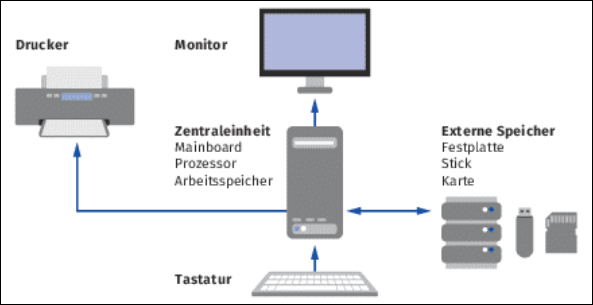
\includegraphics[width=0.5\textwidth]{./images/2.1.1_konfiguration.png}
        \caption{EVA-Prinzip Beispiel}\label{fig:EVA-Prinzip}
    \end{figure}\\
    Konfiguration:\\
    Bezeichnung für abgestimmte Zusammenstellung von Hardware und Software auf Nutzungszweck des Kunden.
\subsection{Bedeutende Entwicklungsschritte in der Computertechnik}
    TODO
\subsection{Entwicklungstrends präsentieren}
    TODO
\subsection{Komponentenhersteller und Systemarchitekturen präsentieren}
    TODO

\section{Das Leistungsportfolio im Ausbildungsbetrieb präsentieren}
\subsection{Arbeitsplätze und Arbeitsumgebungen für IT-Systeme beschreiben}
    TODO
\subsection{Marktgängige IT-Systeme vorstellen}
    TODO
\subsection{Das Leistungsportfolio im IT-Bereich präsentieren}
    TODO

\section{Auswahlkriterien zu IT-Produkten allgemein unterscheiden}
\subsection{Qualität und Leistungsfähigkeit von IT-Systemen und IT-Services beschreiben}
    TODO

\subsection{Umweltschutz und Green-IT als wichtige IT-Ziele darstellen}
    TODO
\subsection{Wirtschaftlichkeit von IT-Systemen erläutern}
    TODO
\subsection{IT-Sicherheit von IT-Systemen, Informations- und Datenschutz erläutern}
    TODO
\subsection{IT-Sicherheit von IT-Systemen, Informations- und Datenschutz erläutern}
    TODO

\end{document}